\documentclass[a4paper, 11pt]{article}
\usepackage[polish]{babel}
\usepackage[T1]{fontenc}
\usepackage{hyperref}
\usepackage{array}
\usepackage{amssymb}
\hypersetup{
    colorlinks,
    citecolor=black,
    filecolor=black,
    linkcolor=black,
    urlcolor=black
}
\usepackage{graphicx}

\usepackage{tikz}
\usetikzlibrary{fit,arrows,matrix,positioning, calc, shapes.gates.logic.IEC, shapes.gates.logic.US}
\tikzstyle{branch}=[fill,shape=circle,minimum size=3pt,inner sep=0pt]


\title{%
       \large Sprawozdanie Laboratorium Mikroelektronika \\
       \huge Obsługa programu LTSpice}

\author{Stanisław Fiedler 160250}
\date{LAB 1, 15 października 2024}

\begin{document}

\maketitle
\tableofcontents

\section{Zadanie 1}

\subsection{Wyjaśnić czym różni się analiza Transient od analizy stałoprądowej DC.}\label{sub:1.1} % (fold)

Analiza transient przedstawia zmianę badanej wartości w układzie względem czasu. Analiza stałoprądowa DC pozwala zbadać wartość napięcia w badanym miejscu względem napięcia podawanego na układ.

% subsection 1.1 (end)

\pagebreak

\section{Zadanie 2}

\subsection{Przedstawić wyniki symulacyjne oraz wyjaśnić zasadę działania obwodu.}\label{sub:2.1} % (fold)

\begin{figure}[h]
	\centering
	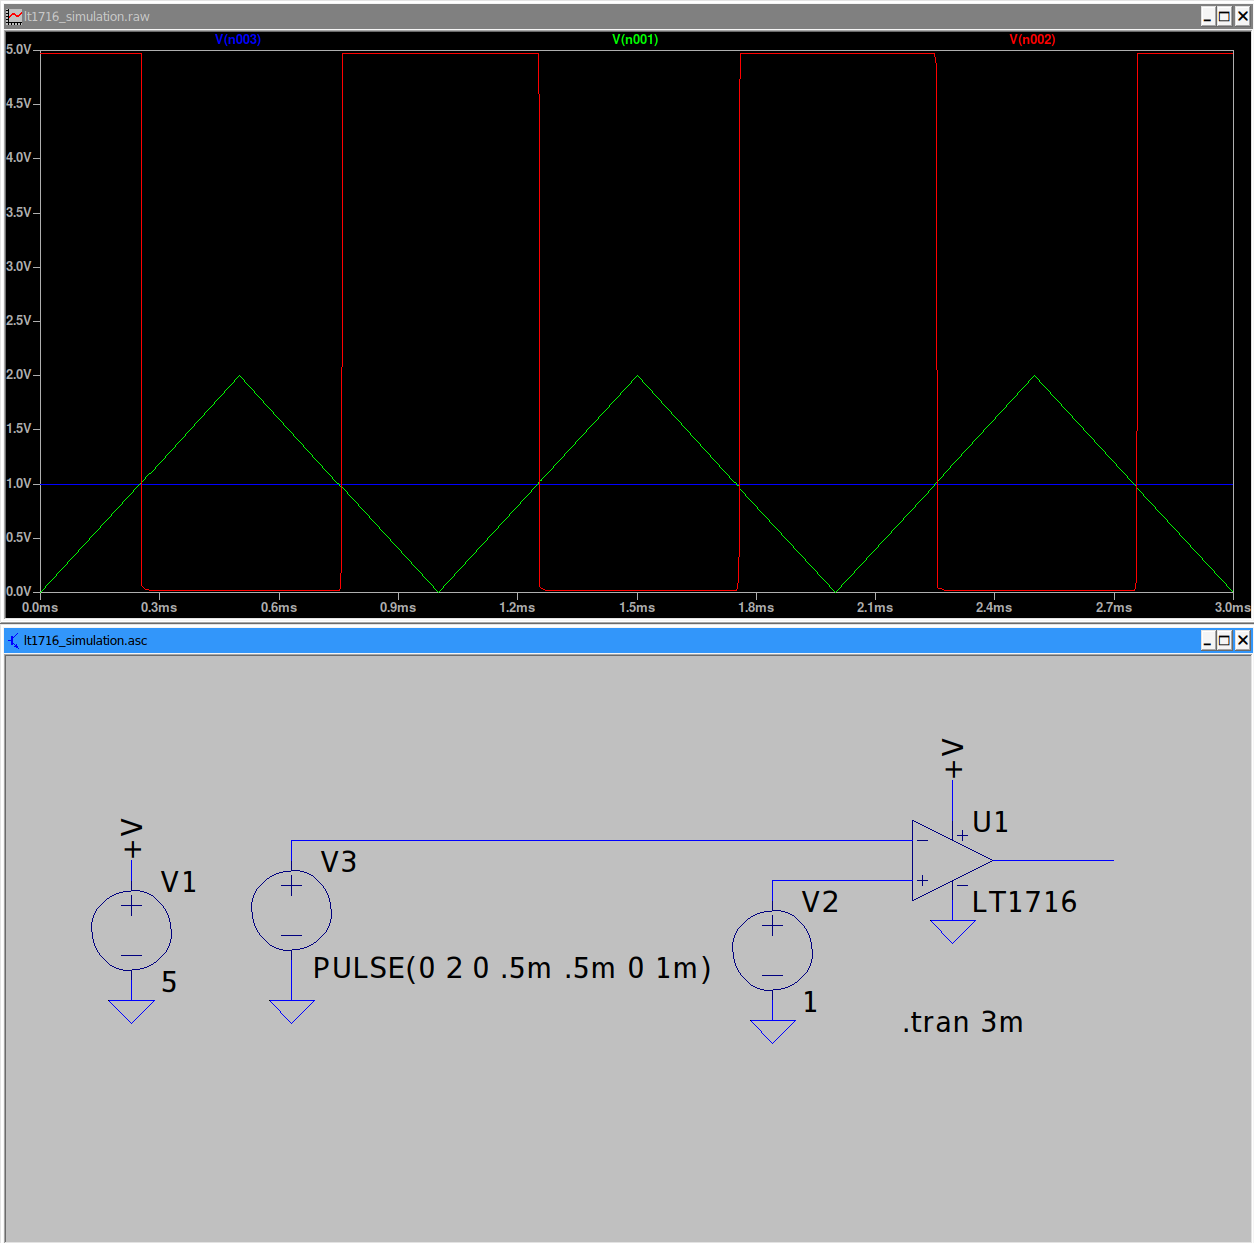
\includegraphics[scale = 0.25]{images/21_simulation.png}
	\caption{Symulacja 1}
	\label{fig:sim1}
\end{figure}


Jeżeli napięcie V3 będzie wyższe niż napięcie V2 to napięcie na wyjściu komparatora będzie wynosiło 0V. W sytuacji odwrotnej, kiedy napięcie V2 będzie wyższe niż V3 napięcie na wyjściu będzie wynosić V+.


W obwodzie symulacji \ref{fig:sim1} napicie V2 wynosi 1V, a V3 zmienia się w czasie od 0V do 2V. Kiedy napięcie V3 przekracza 1V na wyjście podawane jest 0V, w pozostałym czasie na wyjściu jest 5V.

% subsection 2.1 (end)

\pagebreak

\subsection{Zaproponować dowolną zmianę w obwodzie. Opisać wprowadzoną zmianę oraz przedstawić dla
	niej wyniki symulacyjne.}\label{sub:2.2} % (fold)

\begin{figure}[h]
	\centering
	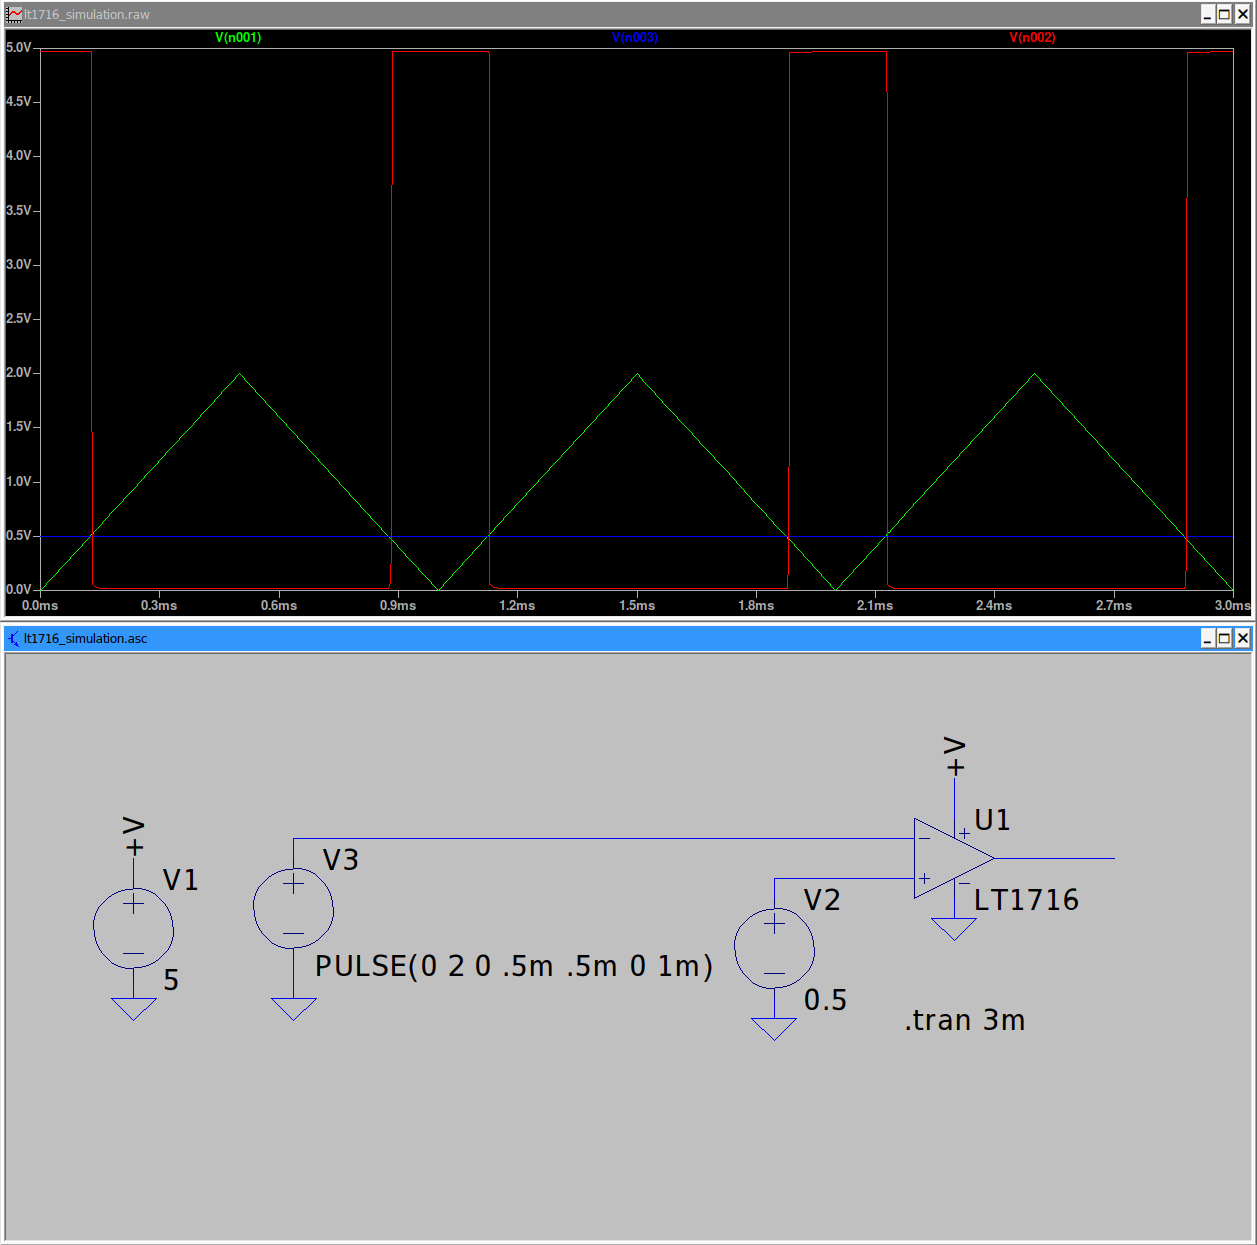
\includegraphics[scale = 0.25]{images/22_simulation.png}
	\caption{Symulacja 2}
	\label{fig:sim2}
\end{figure}

W obwodzie symulacji \ref{fig:sim2} napięcie V2 zostało zmienione na 0,5V. Zmiana ta spowodowała że napięcie 5V na wyjściu komparatora jest tylko kiedy napięcie V3 spada poniżej 0,5V. Przez pozostały czas wynosi ono 0V.

% subsection 2.2 (end)

\end{document}

